%; whizzy chapter
% -initex iniptex -latex platex -format platex -bibtex jbibtex -fmt fmt
% $B0J>e(B whizzytex $B$r;HMQ$9$k>l9g$N@_Dj!#(B

%     Tokyo Debian Meeting resources
%     Copyright (C) 2007 Junichi Uekawa

%     This program is free software; you can redistribute it and/or modify
%     it under the terms of the GNU General Public License as published by
%     the Free Software Foundation; either version 2 of the License, or
%     (at your option) any later version.

%     This program is distributed in the hope that it will be useful,
%     but WITHOUT ANY WARRANTY; without even the implied warranty of
%     MERCHANTABILITY or FITNESS FOR A PARTICULAR PURPOSE.  See the
%     GNU General Public License for more details.

%     You should have received a copy of the GNU General Public License
%     along with this program; if not, write to the Free Software
%     Foundation, Inc., 51 Franklin St, Fifth Floor, Boston, MA  02110-1301 USA


%   Pdf$B:n@.<j=g(B
% dvipdfmx debianmeetingresume200606.dvi
%  preview (shell-command (concat "xpdf " (replace-regexp-in-string "tex$" "pdf"(buffer-file-name)) "&"))
% $B2hA|%U%!%$%k$r=hM}$9$k$?$a$K$O(Bebb$B$rMxMQ$7$F(Bboundingbox$B$r:n@.!#(B
%(shell-command "cd image200606; ebb *.png")

%%$B$3$3$+$i%X%C%@3+;O!#(B

\documentclass[mingoth,a4paper]{jsarticle}
\usepackage[dvipdfm]{graphicx}
\usepackage{fancybox}
\usepackage{longtable}
\usepackage{ascmac}	% $B0O$_(B (screen,itembox)
\usepackage{fancyvrb}   % $B0O$_(B Verbatim $B$N$?$a$KI,MW(B
\usepackage[dvipdfm]{hyperref}
\usepackage{url}
\usepackage[dvipdfm]{color}
\usepackage{wrapfig} % $B?^$N$^$o$j$3$_(B
\usepackage{nextpage}

% $BF|IU$rDj5A$9$k!"Kh7nJQ$o$j$^$9!#(B
\newcommand{\debmtgyear}{2007}
\newcommand{\debmtgdate}{19}
\newcommand{\debmtgmonth}{5}
\newcommand{\debmtgnumber}{28}

%http://www.naney.org/diki/dk/hyperref.html
%$BF|K\8l(BEUC$B7O4D6-$N;~(B
\AtBeginDvi{\special{pdf:tounicode EUC-UCS2}}
%$B%7%U%H(BJIS$B7O4D6-$N;~(B
%\AtBeginDvi{\special{pdf:tounicode 90ms-RKSJ-UCS2}}

%% spacing $B$N@_Dj$r$9$k!#30OH$r8:$i$9!#(B
\setlength\headheight{0mm}
\setlength\topmargin{-20mm}
\setlength\headsep{0mm}
\setlength\topskip{3mm}
\setlength\maxdepth{4pt}
\setlength\columnsep{6mm}
\setlength\textheight{252mm}
\setlength\topmargin{-5mm}
\setlength\textwidth{170mm}
\setlength\oddsidemargin{-5mm}
\setlength\evensidemargin{-5mm}

% commandline$B4D6-$rDj5A!#2hLLF~=PNO$K$D$$$F$O(Bcommandline$B4D6-(B
% $B$GI=5-$9$k(B
\newenvironment{commandline}%
{\VerbatimEnvironment
  \begin{Sbox}\begin{minipage}{15cm}\begin{fontsize}{7.3}{7.3} \begin{BVerbatim}}%
{\end{BVerbatim}\end{fontsize}\end{minipage}\end{Sbox}
  \setlength{\fboxsep}{8pt}\fbox{\TheSbox}}


%%% start of santaku
\makeatletter
\newwrite\tf@jqz
\immediate\openout\tf@jqz\jobname.jqz\relax
\makeatother
\newcounter{santakucounter}
\newcommand{\santaku}[5]{%
\addtocounter{santakucounter}{1}

\addtocontents{jqz}{\arabic{santakucounter}. #5\\}
\begin{minipage}{1\hsize}
$BLdBj(B\arabic{santakucounter}. 
#1\\
$B""(B A #2\\
$B""(B B #3\\
$B""(B C #4
\end{minipage}
\hspace{1cm}
\\


}
%%% end of santaku

\newcommand{\emptyspace}{(\underline{\hspace{1cm}})}

\newcommand{\subsubsubsection}[1]{%
\vspace{1zw}{\bf #1}\\}

% section$B$r%;%s%?%j%s%0$9$k(B
\makeatletter
  \renewcommand{\section}{\@startsection{section}{1}{\z@}%
    {\Cvs \@plus.5\Cdp \@minus.2\Cdp}% $BA0%"%-(B
    {.5\Cvs \@plus.3\Cdp}% $B8e%"%-(B
    {\normalfont\Huge\headfont\raggedright\centering}} % style
\makeatother

% section $B$NBe$o$j$N4D6-(B
\newcommand{\dancersection}[2]{%
\newpage
$BEl5~%(%j%"(BDebian$BJY6/2q(B \debmtgyear{}$BG/(B
\hrule
\vspace{0.5mm}
\hrule
%
\vspace{4cm}
\hrule
\vspace{0.5mm}
\hrule
%
\vspace{-7cm}
\begin{minipage}[b]{0.7\hsize}
\section{#1}
\hfill{}#2\\
\vspace{2cm}
\end{minipage}
\begin{minipage}[b]{0.3\hsize}
\hfill{}
\includegraphics[height=8cm]{image200502/openlogo-nd.eps}\\
\end{minipage}
%
%\hfill{}
\includegraphics[width=16cm]{image2006-natsu/guruguru-sand-light.png}\\
\vspace{-1cm}
}

% BTS$B$NHV9f$r8+$k$?$a$N%3%^%s%I(B
\newcommand{\debianbug}[1]{Bug\##1\footnote{\url{http://bugs.debian.org/#1}}}

% for dancerj
\newcommand{\fgref}[1]{$B?^(B\ref{#1}}
\newcommand{\tbref}[1]{$BI=(B\ref{#1}}

\begin{document}

\begin{titlepage}

\includegraphics[height=252mm]{image2007-natsu/2007-summer.eps}

%\thispagestyle{empty}
\end{titlepage}

\newpage
\setcounter{tocdepth}{1}
\tableofcontents
\vspace{6cm}

\large
\begin{itembox}{\bf$B!X$"$s$I$-$e$a$s$F$C$I(B $B$G$S$"$s!Y$K$D$$$F(B}
$BK\=q$O!"El5~<~JU$GKh7n9T$J$o$l$F$$$k!XEl5~%(%j%"(B Debian $BJY6/2q!Y$G(B
$B;HMQ$5$l$?;qNA!&>.%M%?!&I,;&5;$J$I$r0l:}$K$^$H$a$?$b$N$G$9!#(B
$B<}O?HO0O$OJY6/2qBh(B18$B2s$+$iBh(B22$B2s$^$G!#(B
$BFbMF$OL5J]>Z!"$D$C$3$_$J$I$,$"$l$PJY6/2q$K$F!#(B
\end{itembox}
\normalfont



\newpage
\dancersection{Debian Weekly News trivia quiz}{$B>e@n=c0l(B}

$B$H$3$m$G!"(BDebian Weekly News (DWN)$B$OFI$s$G$$$^$9$+!)(B
Debian $B3&7($G$*$-$F$$$k$3$H$K$D$$$F=q$$$F$$$k(BDebian Weekly News.
$BKh2sFI$s$G$$$k$H$$$m$$$m$HJ,$+$C$FMh$^$9$,!"0l?M$GFI$s$G$$$F$b!"2r@b$,>/(B
$B$J$$$N$G!"(B
$B0UL#$,$o$+$i$J$$$H$3$m$b$"$k$+$bCN$l$^$;$s!#$_$s$J$G(BDWN$B$rFI$s$G$_$^$7$g$&!#(B

$BL!A3$HFI$`$@$1$G$O$*$b$7$m$/$J$$$N$G!"(BDWN$B$N5-;v$+$i=PBj$7$?0J2<$N<ALd$K$3$?$($F$_$F$/$@$5$$!#(B
$B8e$GFbMF$O2r@b$7$^$9!#(B


\subsection{2006$BG/(B41$B9f(B}
\url{http://www.debian.org/News/weekly/2006/41/}



\dancersection{Debian Weekly News $BLdBj2sEz(B}{$B>e@n(B}
%\twocolumn

Debian Weekly News $B$NLdBj2sEz$G$9!#(B
$B$"$J$?$O2?Ld$o$+$j$^$7$?$+!)(B
%$B2sEz$O(Bdebianmeetingresume2007-natsu.jqz$B$H$$$&%U%!%$%k$K@8@.$5$l$k$N$G!"(B
%$B$=$l$r<jF0$G%3%T%Z$7$F;H$&!#(B
\\
% $B$3$3$+$i%3%T%Z(B
\onecolumn

\cleartooddpage

\vspace*{15cm}
\hrule
\vspace{2mm}

\includegraphics[width=2cm]{image200502/openlogo-nd.eps}
\noindent \Large \bf $B$"$s$I$-$e$a$s$F$C$I(B $B$G$S$"$s(B 2007$BG/2F9f(B\\ \\
\noindent \normalfont 2007$BG/(B8$B7n(B15$BF|(B \hspace{5mm}  $B=iHGBh(B1$B:~H/9T(B\\
\noindent \normalfont $BEl5~%(%j%"(B Debian $BJY6/2q(B $B!JJT=8!&0u:~!&H/9T!K(B\\
\hrule

\end{document}
